\input{../../input/main}

\usetikzlibrary{hobby}

\begin{document}

\begin{center}
  \Large{\textbf{Городской центр физического образования, 10 класс.}\\
  \textit{Серия 10, 27 ноября 2014.}}
\end{center}

\begin{center}
  \Large \textbf{ КПД циклов. }
\end{center}

\large


\taskpic{ С 3 молями идеального одноатомного газа совершен цикл,
  изображённый на рисунке. Температуры газа в различных состояниях
  равны: $T_1=400$ К, $T_2=800$ К, $T_3=2400$ К и $T_4=1200$
  К. Найдите работу $A$ газа за цикл. }
{
  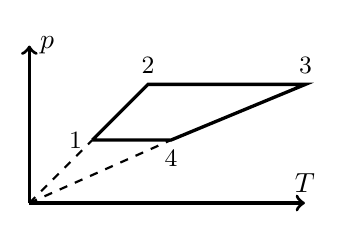
\begin{tikzpicture}
    \draw[very thick,->] (0,0) -- (3.5,0) node[above] {$T$};
    \draw[very thick,->] (0,0) -- (0,2) node[right] {$p$};
    \draw[thick,dashed] (0,0) -- (0.8,0.8) node[left] {\small 1};
    \draw[thick,dashed] (0,0) -- (1.8,0.8) node[below] {\small 4};
    \draw[very thick] (0.8,0.8) -- ++(45:1cm) node[above] {\small 2}
    -- ++(0:2cm) node[above] {\small 3} -- (1.8,0.8) -- (0.8,0.8);  
  \end{tikzpicture}
}


\task{ Идеальный одноатомный газ (количество вещества $\nu$) участвует
  в циклическом процессе, состоящем из двух изотерм и двух изохор. При
  изохорическом нагревании газ получает количество теплоты $Q_1$, а
  при изотермическом расширении --- количество теплоты
  $Q_2$. Минимальная температура газа в данном циклическом процессе
  равна $T_{\mathrm{min}}$. Найдите:
  \begin{enumerate}
  \item максимальную температуру газа;
  \item количества теплоты, отданные газом при изохорическом
    охлаждении и изотермическом сжатии;
  \item работу, совершённую газом на каждой из стадий процесса;
  \item КПД теплового двигателя, работающего по
  рассматриваемому циклу.
  \end{enumerate}
}


\task{ Найдите КПД цикла, состоящего из двух изобар и двух адиабат,
  если в пределах цикла давление изменяется в $n$ раз. Рабочее
  вещество --- одноатомный идеальный газ с показателем адиабаты
  $\gamma$.  }

\taskpic{ С одним молем идеального одноатомного газа совершен цикл,
  изображённый на рисунке (участок (3,1) представляет
  адиабату). Найдите КПД такого цикла. Координаты всех трёх точек
  известны. }
{
  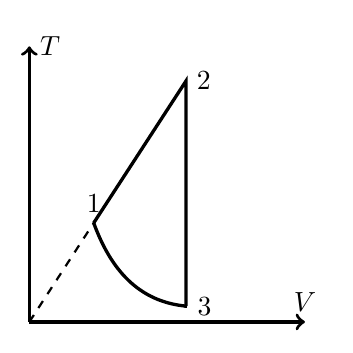
\begin{tikzpicture}
    \draw[very thick,->] (0,0) -- (3.5,0) node[above] {$V$};
    \draw[very thick,->] (0,0) -- (0,3.5) node[right] {$T$};
    \draw[very thick] ({atan(2/1.3)}:1.5cm) node[above] {1}
    to[out=290,in=175] (2,0.2) node[right] {3}; 
    \draw[thick,dashed] (0,0) -- (1.3,2);
    \draw[very thick] ({atan(2/1.3)}:1.5cm) --
    ++({atan(2/1.3)}:2.15cm) node[right] {2} |- (2,0.2); 
  \end{tikzpicture}
}


\end{document}


%%% Local Variables: 
%%% mode: latex
%%% TeX-engine:xetex
%%% TeX-PDF-mode: t
%%% End:
